\section{Results: Independent-Slab Mechanical Evolution}
\label{sec:mechanics-results}
The independent-slab mechanics cohort comprises 24 clot--condition records and 204 slab trajectories, with 13392 saved slab states aggregated into 1512 clot-level observations. Figure~\ref{fig:mechanics-response} shows contraction and cohesive-link development; Table~\ref{tab:mechanics-endpoints} gives the matched 10 min endpoints and the available 30 min endpoints. All times in this section are mechanical model times.

\begin{figure*}[!tp]
\centering
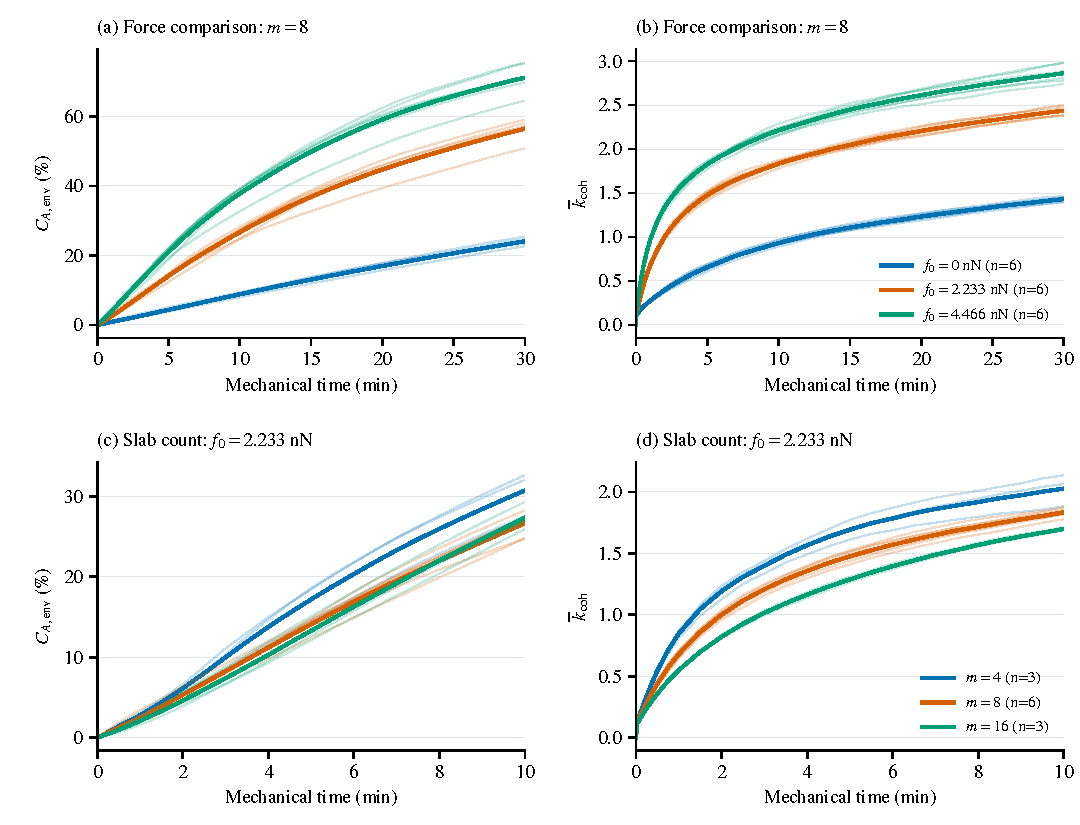
\includegraphics[width=\textwidth]{figures/mechanics_response.pdf}
\caption{Mechanical evolution from saved trajectories. (a,b) Force comparison at $m=8$ through 30 min, with six clot replicas per force. (c,d) Slab-count comparison at $f_0=2.233$ nN through the common 10 min horizon, with three replicas for $m=4$ and 16 and six for $m=8$. Thin curves show individual clots; thick curves show replica means, not fitted responses. Contraction uses the center-position convex-hull envelope, and cohesive degree excludes backbone edges.}
\label{fig:mechanics-response}
\end{figure*}

\begin{table*}[!tp]
\centering
\small
\setlength{\tabcolsep}{6pt}
\renewcommand{\arraystretch}{1.08}
\caption{Mechanical endpoint summaries. Entries are mean $\pm$ sample standard deviation across $n$ clot replicas, not confidence intervals or variability across individual slabs. The $m=4$ records end at 10 min.}
\label{tab:mechanics-endpoints}
\begin{tabular}{@{}rrrrrrr@{}}
\toprule
\shortstack{Time\\(min)} & $m$ & \shortstack{$f_0$\\(nN)} & $n$ & \shortstack{$C_{A,\mathrm{env}}$\\(\%)} & $\overline{k}_{\mathrm{coh}}$ & \shortstack{$q_{\mathrm{att}}$\\(\%)} \\
\midrule
10 & 4 & 2.233 & 3 & $30.7\pm2.8$ & $2.03\pm0.13$ & $100.0\pm0.0$\\
\specialrule{0.2pt}{1.5pt}{1.5pt}
10 & 8 & 0 & 6 & $8.8\pm0.5$ & $0.93\pm0.03$ & $100.0\pm0.0$\\
\specialrule{0.2pt}{1.5pt}{1.5pt}
10 & 8 & 2.233 & 6 & $26.7\pm1.5$ & $1.83\pm0.04$ & $99.6\pm1.1$\\
\specialrule{0.2pt}{1.5pt}{1.5pt}
10 & 8 & 4.466 & 6 & $37.8\pm2.6$ & $2.21\pm0.05$ & $99.4\pm1.4$\\
\specialrule{0.2pt}{1.5pt}{1.5pt}
10 & 16 & 2.233 & 3 & $27.3\pm1.8$ & $1.70\pm0.01$ & $99.8\pm0.2$\\
\midrule
30 & 8 & 0 & 6 & $24.0\pm1.0$ & $1.43\pm0.03$ & $99.8\pm0.4$\\
\specialrule{0.2pt}{1.5pt}{1.5pt}
30 & 8 & 2.233 & 6 & $56.4\pm2.9$ & $2.44\pm0.06$ & $99.8\pm0.5$\\
\specialrule{0.2pt}{1.5pt}{1.5pt}
30 & 8 & 4.466 & 6 & $71.1\pm4.0$ & $2.86\pm0.10$ & $99.9\pm0.3$\\
\specialrule{0.2pt}{1.5pt}{1.5pt}
30 & 16 & 2.233 & 3 & $61.4\pm2.0$ & $2.44\pm0.04$ & $100.0\pm0.0$\\
\bottomrule
\end{tabular}
\end{table*}

\subsection{Force-Dependent Contraction and Cohesion}
At $m=8$, the mean envelope contraction at 30 min increases from 24.0\% at $f_0=0$ to 56.4\% at 2.233 nN and 71.1\% at 4.466 nN. The corresponding mean cohesive degrees are 1.43, 2.44, and 2.86. Thus, the stronger baseline settings accompany both greater envelope shrinkage and more cohesive incidences per node in this sample. The sample standard deviations in Table~\ref{tab:mechanics-endpoints} quantify between-clot variability, not numerical error or uncertainty in a population mean. As specified in Eq.~\eqref{eq:wlctraction}, the zero-baseline setting still retains stiffness-dependent filopodial traction and is not a passive-network control.

\subsection{Comparison Across Slab Counts}
At the common 10 min endpoint and $f_0=2.233$ nN, mean contractions are 30.7\%, 26.7\%, and 27.3\% for $m=4$, 8, and 16, respectively. Mean cohesive degree decreases across those settings from 2.03 to 1.83 to 1.70. The contraction means do not show a monotonic dependence on $m$ over these three settings. This comparison changes the planar platelet and junction populations as well as the slab-count representation, and the replica counts are unequal. It therefore does not isolate a thickness effect or establish mechanical convergence with slab count. The $m=16$ records reach 61.4\% mean contraction at 30 min, whereas no matched 30 min measurement is available for $m=4$.

\subsection{Attachment Occupancy and Continuing Evolution}
Filopodial attachment is nearly saturated at the reported endpoints, with mean occupied fractions between 99.4\% and 100\%. For the $m=8$, $f_0=2.233$ nN condition, all arms are attached by the first saved 1 s frame. This does not imply persistent attachment to the same nodes or constant force per arm. Mechanical reorganization continues after occupancy saturates: from 25 to 30 min, mean contraction increases by a further 3.4, 5.4, and 5.2 percentage points at $f_0=0$, 2.233, and 4.466 nN, respectively. Accordingly, the 30 min endpoints are finite-time observations, not demonstrated mechanical equilibria.

\subsection{Independent Slabs Compared with Sections of Three Volumetric Clots}
\label{sec:virtual-comparison}
The independent and projected slabs differed before contraction began. The mean initial number of platelet profiles per slab was similar (9 in the independent model; $8.3\pm0.2$ in the 3D sections), but the initial projected backbone length per slab was $986\pm17~\mu\mathrm m$ in the independent stacks versus $2028\pm28~\mu\mathrm m$ in the 3D sections. These lengths describe projected centerlines, not fibrin mass. All spreads below are sample standard deviations across complete clots.

\begin{figure}[!tbp]
\centering
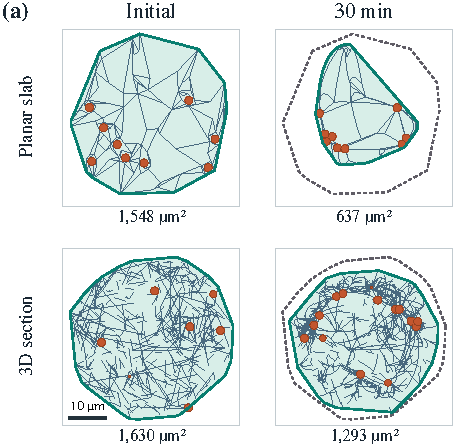
\includegraphics[width=\linewidth]{figures/representative_envelopes.pdf}\par
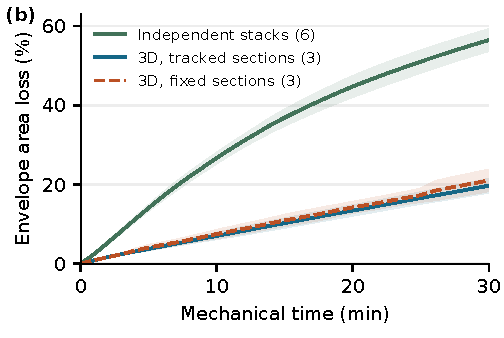
\includegraphics[width=\linewidth]{figures/mechanics_three_clots.pdf}
\caption{Projected envelope contraction. (a) Independent slab 5 of stack 1 and the fixed $0\le z<4~\mu\mathrm m$ section of 3D clot 1, at the same scale. Shading is the convex hull of fibrin nodes and platelet centers; dashed outlines mark the initial envelopes. (b) Area loss summed over eight slabs per clot. Lines and bands are means and sample SDs across six independent stacks or three volumetric clots. The two 3D curves follow the same material or the same depths.}
\label{fig:virtual-sections}
\end{figure}
By 10~min, tracked material in the 3D clots had lost $7.0\pm0.9$\% of its projected envelope area, compared with $26.7\pm1.5$\% in the independent stacks (Fig.~\ref{fig:virtual-sections}). By 30~min, those losses were $19.7\pm1.9$\% and $56.4\pm2.9$\%, respectively. Fixed-depth sections of the same three volumetric clots gave $21.0\pm2.8$\% loss at 30~min; 36, 29 and 28 of their 45 platelet centers ended in a different section from where they began.

The contrast extended beyond the hull. At 30~min the in-plane fibrin-node radius had decreased by $14.9\pm0.7$\% in tracked 3D sections and $30.9\pm1.5$\% in independent stacks. The fraction of backbone length overlapping platelet profiles rose from $1.6\pm0.2$\% to $19.2\pm1.6$\% in fixed 3D sections and from zero to $59.0\pm1.3$\% in independent slabs.
